\documentclass[a4paper]{article}

\usepackage[utf8]{inputenc}
\usepackage{a4wide}
\usepackage{indentfirst}
\usepackage{hyperref}
\usepackage[capitalise]{cleveref}
\usepackage{minted}
\usepackage{graphicx}
\usepackage{float}
\usepackage{witharrows}

\AtBeginEnvironment{minted}{\let\itshape\relax}

\begin{document}

\section*{Exercise 1}

To show that $(m_1, m_2) = (m'_1, m'_2)$, we have to show that
$m_1 \equiv x_T^{-1} c_1 \ (\mathrm{mod} \ p)$ and $m_2 \equiv y_T^{-1}c_2 \ (\mathrm{mod} \ p)$.

\vspace{\baselineskip}

\[
\setlength{\jot}{10pt}
\begin{WithArrows}
m_1 \equiv x_T^{-1} c_1 \ (\mathrm{mod} \ p) \ &\wedge \ m_2 \equiv y_T^{-1} c_2 \ (\mathrm{mod} \ p) \Arrow{$c_1 \equiv x_Sm_1 \ (\mathrm{mod} \ p)$ and \\$c_2 \equiv y_Sm_2 \ (\mathrm{mod} \ p)$} \\
m_1 \equiv x_T^{-1} x_Sm_1 \ (\mathrm{mod} \ p) &\wedge m_2 \equiv y_T^{-1} y_Sm_2 \ (\mathrm{mod} \ p)
\end{WithArrows}
\]

\vspace{\baselineskip}

For $(m_1, m_2) = (m'_1, m'_2)$ to hold, we just have to show that $T^{-1}S \equiv 1 \ (\mathrm{mod} \ p)$.

\[ 
\setlength{\jot}{10pt}
\begin{WithArrows}
        &\Arrow{$T = n_AR$ and $S = kQ_A$}\\
T^{-1}S &\equiv (n_AR)^{-1}kQ_A \ (\mathrm{mod} \ p) \Arrow{$R = kP$ and $Q_A = n_AP$} \\
        &\equiv n_A^{-1}(kP)^{-1}kn_AP \ (\mathrm{mod} \ p) \Arrow{$n_An_A^{-1} = 1$, $kk^{-1} = 1$\\ and $PP^{-1} = 1$} \\
        &\equiv 1 \ (\mathrm{mod} \ p)
\end{WithArrows}
\]

\vspace{\baselineskip}

Thus, $(m_1, m_2) = (m'_1, m'_2)$.

\section*{Exercise 2}

\vspace{\baselineskip}

\begin{minted}{py}
from sage.all import *

def gen_pub_key(A, B, p, x_p, y_p):
    Fp = FiniteField(p)
    E = EllipticCurve(Fp, [A, B])
    assert(E.is_on_curve(x_p, y_p))

    P = E([x_p, y_p])
    n_a = ZZ(Fp.random_element())
    Q_A = n_a * P

    return (Q_A, n_a)


def encrypt(A, B, p, x_p, y_p, Q_A, m_1, m_2):
    Fp = FiniteField(p)
    E = EllipticCurve(Fp, [A, B])
    assert(E.is_on_curve(x_p, y_p))

    P = E([x_p, y_p])
    k = ZZ(Fp.random_element())
    R = k * P

    S = k * Q_A
    c_1 = (S[0] * m_1) % p
    c_2 = (S[1] * m_2) % p

    return (R, c_1, c_2)
\end{minted}

\begin{minted}{py}
def decrypt(A, B, p, x_p, y_p, R, n_a, c_1, c_2):
    Fp = FiniteField(p)
    E = EllipticCurve(Fp, [A, B])
    assert(E.is_on_curve(x_p, y_p))

    T = n_a * R
    m_1 = (T[0] ** (-1) * c_1) % p
    m_2 = (T[1] ** (-1) * c_2) % p

    return (m_1, m_2)
\end{minted}

\vspace{2\baselineskip}

Running this functions with the Curve P-384, we can see the functions are defined
correctly (\cref{fig:sage}).

\vspace{\baselineskip}

\begin{figure}[H]
    \centering
    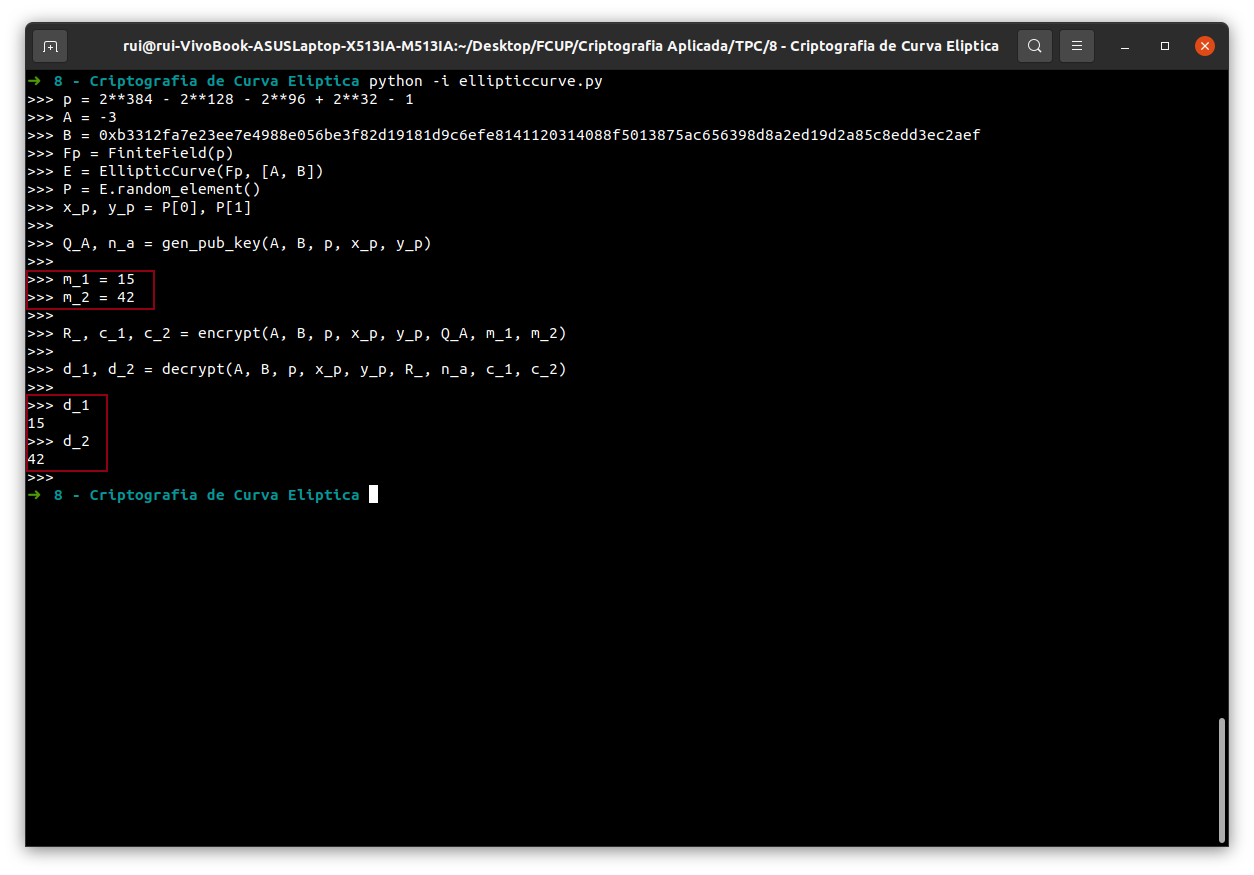
\includegraphics[width=\textwidth]{img/ex2.png}
    \caption{Menezes–Vanstone variant for ECC ElGamal}
    \label{fig:sage}
\end{figure}

\end{document}
